\chapter{\label{cha:sts_siamese_neural_networks}Siamese Neural Networks for STS}

\section{Introduction}
\cite{ranasinghe-etal-2019-semantic}
\textit{Siamese Neural Networks}



We address four research questions in this chapter:

\textbf{RQ1:} Can existing state-of-the-art Siamese neural network architecture be modified to provide better STS results?

\textbf{RQ2:} Can the method further improved with transfer learning and data augmentation techniques?

\textbf{RQ3:} Can the proposed Siamese neural network be easily adopted in to different languages?

\textbf{RQ4:} How well the proposed Siamese neural network perform in a different domain? 


The main contributions of this chapter are as follows.

\begin{enumerate}
	\item We propose a GRU based Siamese neural network that outperforms state-of-the-art LSTM based Siamese neural network in small STS datasets. 
	
	\item We propose a LSTM and Self-attention based Siamese neural network that outperforms state-of-the-art LSTM based Siamese neural network in large STS datasets.
	
	\item We propose further enhancements to the architecture using transfer learning and data augmentation.  
	
	\item We evaluate how well the proposed Siamese neural network architecture performs in different languages and domains. 
	
	\item The initial findings of this chapter is published in \citet{ranasinghe-etal-2019-semantic}. 
	
	\item The code and the pretrained models are publicly available to the community\footnote{The public GutHub repository is available on \url{https://github.com/tharindudr/Siamese-recurrent-rrchitectures}}
\end{enumerate}

\section{Related Work}

\section{Exploring Siamese Neural Networks for STS}

The basic structure of the Siamese neural network architecture used in our experiments is shown in Figure \ref{fig:siamese}. It consists of an embedding layer which represents each sentence as a sequence of word vectors. This sequence of word vectors is fed into a Recurrent Neural Network (RNN) cell which learns a mapping from the space of variable length sequences of 300-dimensional vectors into a 50 dimensional vector. The sole error signal backpropagated during training, stems from the similarity between these 50 dimensional vectors, which can be also used as a sentence representation. Initially, the similarity function we used was based on Manhattan distance. To make sure that the prediction is between 0 and 1, we took the exponent of the negative Manhattan distance between 2 sentence representations. The similarity function was adopted from \citet{Mueller_Thyagarajan_2016}. The proposed variants of our architecture are:


\begin{figure}[ht]
	\centering
	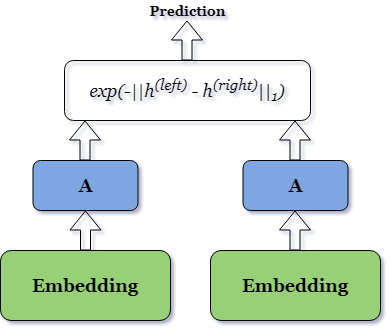
\includegraphics[scale=0.5]{figures/semantic_textual_similarity/siamese_neural_networks/siamese_architecture.png}
	\caption{Basic structure of the Siamese neural network. Unit A is changed over the architectures.}
	\label{fig:siamese}
\end{figure}

\begin{enumerate}
	\item LSTM - Block A in Figure \ref{fig:siamese} contains a single LSTM cell. This is the architecture suggested by \citet{Mueller_Thyagarajan_2016} 
	
	\item Bi-directional LSTM - Block A in Figure \ref{fig:siamese} contains a single Bi-directional LSTM cell. Bi-directional LSTM tends to understand the context better than Unidirectional LSTM \cite{650093}.
	
	\item GRU - Block A in Figure \ref{fig:siamese} contains a single GRU cell. GRUs have been shown to exhibit better performance on smaller datasets \cite{Chung2014EmpiricalEO}. 
	
	\item Bi-directional GRU - Block A in Figure \ref{fig:siamese} contains a single Bi-directional GRU cell. Bi-directional GRUs tend to understand the context better than Unidirectional GRU ~\cite{vukotic:hal-01351733}.
	
	\item LSTM + Attention - Block A in Figure \ref{fig:siamese} contains a single LSTM cell with self attention \cite{NIPS2017_3f5ee243}.
	
	\item GRU + Attention - Block A in Figure \ref{fig:siamese} contains a single GRU cell with self attention \cite{NIPS2017_3f5ee243}.
	
	\item GRU + Capsule + Flatten - Block A in Figure \ref{fig:siamese} contains a GRU followed by a capsule layer and a flatten layer. Dynamic routing used between capsules performs better than a traditional max-pooling layer \cite{NIPS2017_2cad8fa4}.
	
\end{enumerate}
	
	
	As the word embedding model we used Word2vec embeddings \cite{DBLP:journals/corr/abs-1301-3781} pre-trained on Google new corpus\footnote{Pretrained Word2vec can be downloaded from \url{https://code.google.com/archive/p/word2vec/}}. We represented each word as a 300 lengthened vector using this model. For the words that do not appear in this model we used a random vector. We evaluated all the above variations in 
	the three English STS datasets we introduced in \ref{cha:introduction}; SICK, STS 2017 and QUORA. The results are shown in Table \ref{tab:sick_siamese}, Table \ref{tab:sts_siamese} and Table \ref{tab:quora_siamese} respectively. 
	
	 
	\begin{table*}[htb]
		%\footnotesize
		\centering
		\scalebox{0.95}{
			\begin{tabular}{|l|cc|}
				\hline
				\textbf{Model} & $\bm{\rho}$   & $\bm{\tau}$     
				\\ \hline
				\textit{LSTM}                  
				& 0.802 & 0.733  \\
				\textit{Bi-LSTM}                     
				& 0.784 & 0.708   \\
				\textit{GRU}                     
				& 0.838$^{\dagger}$ & 0.780$^{\dagger}$  \\
				\textit{Bi-GRU}                     
				& 0.832 & 0.773  \\
				\textit{LSTM + Attention}                     
				& 0.827  & 0.765       \\
				\textit{GRU + Attention}                     
				& 0.818  & 0.751       \\
				\textit{GRU + Capsule + Flatten}                     
				& 0.806  & 0.733       \\
				\hline
			\end{tabular}
		}
		\caption[Results for SICK with Siamese Neural Network]{Results for SICK dataset with different variants of Siamese Neural Network. For each variant, Pearson Correlation ($\bm{\rho}$) and Spearman Correlation ($\bm{\tau}$) are reported between the predicted values and the gold labels of the test set. Best result from all the variations is marked with ${\dagger}$.}  
		\label{tab:sick_siamese}
	\end{table*}
	
	
	\begin{table*}[htb]
		%\footnotesize
		\centering
		\scalebox{0.95}{
			\begin{tabular}{|l|cc|}
				\hline
			\textbf{Model} & $\bm{\rho}$   & $\bm{\tau}$     
			\\ \hline
			\textit{LSTM}                  
			& 0.831 & 0.762  \\
			\textit{Bi-LSTM}                     
			& 0.784 & 0.708   \\
			\textit{GRU}                     
			& 0.853$^{\dagger}$ & 0.811$^{\dagger}$  \\
			\textit{Bi-GRU}                     
			& 0.832 & 0.773  \\
			\textit{LSTM + Attention}                     
			& 0.827  & 0.765       \\
			\textit{GRU + Attention}                     
			& 0.818  & 0.751       \\
			\textit{GRU + Capsule + Flatten}                     
			& 0.806  & 0.733       \\
			\hline
			\end{tabular}
		}
		\caption[Results for STS 2017 with Siamese Neural Network]{Results for STS 2017 dataset with different variants of Siamese Neural Network. For each variant, Pearson Correlation ($\bm{\rho}$) and Spearman Correlation ($\bm{\tau}$) are reported between the predicted values and the gold labels of the test set. Best result from all the variations is marked with ${\dagger}$. }  
		\label{tab:sts_siamese}
	\end{table*}
	
	
	\begin{table*}[htb]
		%\footnotesize
		\centering
		\scalebox{0.95}{
			\begin{tabular}{|l|c|}
				\hline
				\textbf{Model} & RMSE     
			\\ \hline
			\textit{LSTM}                  
			& 0.802   \\
			\textit{Bi-LSTM}                     
			& 0.784    \\
			\textit{GRU}                     
			& 0.838$^{\dagger}$  \\
			\textit{Bi-GRU}                     
			& 0.832   \\
			\textit{LSTM + Attention}                     
			& 0.827        \\
			\textit{GRU + Attention}                     
			& 0.818       \\
			\textit{GRU + Capsule + Flatten}                     
			& 0.806        \\
			\hline
			\end{tabular}
		}
		\caption[Results for QUORA with Siamese Neural Network]{Results for QUORA dataset with different variants of Siamese Neural Network. For each variant, Pearson Correlation ($\bm{\rho}$) and Spearman Correlation ($\bm{\tau}$) are reported between the predicted values and the gold labels of the test set. Best result from all the variations is marked with ${\dagger}$. }  
		\label{tab:quora_siamese}
	\end{table*}
	
As can be seen in Table \ref{tab:sick_siamese} and \ref{tab:sts_siamese}, for SICK and STS 2017 datasets, GRU based Siamese neural network model outperformed the LSTM based Siamese neural network model which we used as a baseline. It is clear that for the smaller datasets GRU based architecture performs better because GRU has less parameters than LSTM \cite{Chung2014EmpiricalEO}. Furthermore, complex architectures that involves Bi-directional RNNs, Attention and Capsule mechanisms did not perform well compared to the simple architectures like GRU. 

			
\subsection{Impact of Transfer Learning}
Transfer learning is a machine learning method where a model developed for a task is reused as the starting point for a model on a second task. It is a popular approach in deep learning where pre-trained models are used as the starting point for a new task.  	 


	
\subsection{Impact of Data Augmentation}	


\section{Portability to Other Languages}

\section{Portability to Other Domains}

\section{Recent Developments}
The current state-of-the-art in STS with Siamese Neural Network is Sentence-bert \cite{reimers-gurevych-2019-sentence}.

\section{Conclusions}